
\setcounter{chapter}{4}
\chapter{Adição e subtração de frações }

\section{EXPLORANDO O ASSUNTO }

\setcounter{subsection}{0}
\begin{atividade}{}


Miguel e Alice estão participando de uma campanha da escola para coleta de óleo de cozinha. O objetivo é disponibilizar recipientes para que as pessoas depositem óleo. Depois esses recipientes serão destinados a empresas que usarão o óleo descartado para fazer sabão. Eles conseguiram diferentes recipientes e agora desejam saber qual tem maior capacidade.

\begin{center}
\begin{tabular}{ccc}
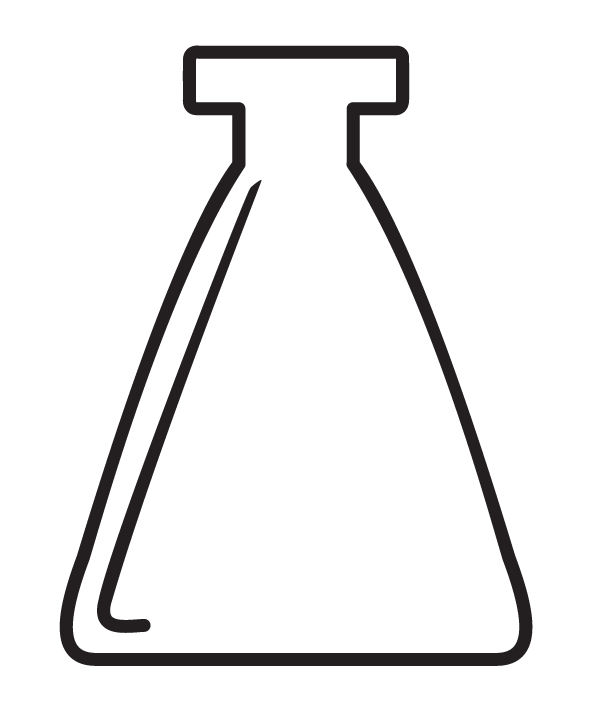
\includegraphics[width=100pt, keepaspectratio]{../figuras/licao05/ativ1_fig01.png} &\quad \quad&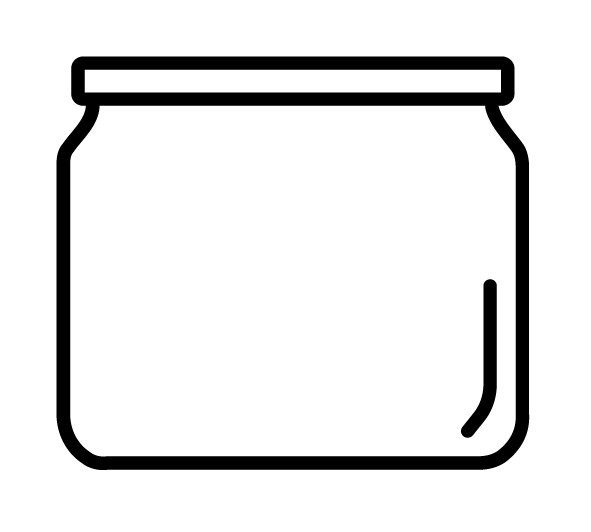
\includegraphics[width=100pt, keepaspectratio]{../figuras/licao05/ativ1_fig02.png}\\ \\
{\bf Recipiente 1:} trazido pela Alice & & {\bf Recipiente 2:} trazido pelo Miguel
\end{tabular}
\end{center}
\vspace{.2cm}

Eles tiveram a seguinte ideia: encheram os dois recipientes com água para, depois, verificar onde havia mais água. Para isso, usaram um copo como unidade de medida.
\begin{itemize}
 \item O recipiente trazido por Alice foi enchido com 26 copos.
 \item O recipiente trazido por Miguel foi enchido com 40 copos.
\end{itemize}
Eles então observaram que a partir de {\bf uma unidade de medida comum} (nesse caso o copo), poderiam não só dizer qual recipiente tinha maior capacidade, mas também o quanto era maior e qual seria a capacidade dos dois recipientes juntos.
Usando a ideia de medida de Miguel e Alice, isto é, tomando o copo como unidade de medida, responda:
  \begin{enumerate}[a)]
   \item Qual recipiente tem maior capacidade?
   \item Qual é a capacidade dos dois recipientes juntos?
   \item Quanta água se deve retirar do recipiente maior para que sobre a mesma quantidade de água que há no recipiente menor?
  \end{enumerate}
\end{atividade}

\begin{atividade}[label=chap5-ativ2]{}


A professora Estela quer enfeitar sua sala de aula para uma festa da escola. Para isso ela comprou várias fitas, todas de mesmo tamanho, nas cores vermelho, azul e amarelo.

\begin{center}
\begin{tikzpicture}[x=1.0cm,y=1.0cm, scale=.5]
\draw[fill=attention] (0.,1) rectangle (12.,3.);
\draw[fill=common] (0.,-2) rectangle (12.,0.);
\draw[fill=light] (0.,-5) rectangle (12.,-3.);
\end{tikzpicture}
\end{center}


A professora cortou cada fita vermelha em 3 partes iguais, cada fita azul em 2 partes iguais e cada fita amarela em 4 partes iguais.

\begin{center}
\begin{tikzpicture}[x=1.0cm,y=1.0cm, scale=.5]
\draw[fill=attention] (0.,1) rectangle (12.,3.);
\foreach \x in {4,8} \draw[dashed] (\x,1) -- (\x,3);
\draw[fill=common] (0.,-2) rectangle (12.,0.);
\draw[dashed] (6,-2) -- (6,0);
\draw[fill=light] (0.,-5) rectangle (12.,-3.);
\foreach \x in {3,6,9} \draw[dashed] (\x,-5) -- (\x,-3);
\end{tikzpicture}
\end{center}

\begin{enumerate} [\quad a)] %s
  \item     A que fração da fita original corresponde cada pedaço recortado pela professora Estela?
 \end{enumerate}

 Em seguida, a professora Estela começou a juntar pedaços recortados das fitas, formando novas fitas coloridas. Ela começou juntando (de forma intercalada) um pedaço azul e dois pedaços amarelos.     \mbox{} \newline

\begin{center}
\begin{tikzpicture}[x=1.0cm,y=1.0cm, scale=.5]
\draw[fill=light] (0.,0) rectangle (3,2);
\draw[fill=common] (3,0) rectangle (9.,2.);
\draw[fill=light] (9,0) rectangle (12,2);
\end{tikzpicture}
\end{center}

Ela verificou que a nova fita formada tinha o mesmo tamanho da fita original. Isso aconteceu porque cada pedaço azul tem o mesmo tamanho de dois pedaços amarelos. Podemos representar o tamanho da nova fita formada pela professora por meio de uma {\bf soma de frações}. Cada pedaço azul corresponde a $\frac{1}{2}$ da fita original. Cada pedaço amarelo corresponde a $\frac{1}{4}$ da fita original, então 2 pedaços amarelos correspondem a $\frac{2}{4}$ da fita original. Portanto, o tamanho da nova fita é igual a: $$\dfrac{1}{2} + \dfrac{2}{4}.$$ Mas, como $\frac{2}{4}$ é igual a $\frac{1}{2}$ (cada pedaço azul tem o mesmo tamanho de dois pedaços amarelos), então: $$\dfrac{1}{2} + \dfrac{2}{4} = \dfrac{1}{2} + \dfrac{1}{2}.$$ O resultado dessa soma $\frac{1}{2} + \frac{1}{2}$ é igual 2 pedaços de $\frac{1}{2}$, isto é, $\frac{2}{2}$ (que é igual 1). Assim: $$\dfrac{1}{2} + \dfrac{2}{4} = \dfrac{1}{2} + \dfrac{1}{2} = 1.$$ Neste caso, o resultado 1 corresponde ao tamanho da fita original.
 \begin{enumerate} [\quad a)] %s
 \item[\quad b)]    A professora também agrupou pedaços de fita, juntando 1 pedaço amarelo e 1 pedaço azul, como na figura a seguir. A qual fração do tamanho original das fitas esses dois pedaços juntos correspondem?
\end{enumerate} %s

%\begin{center}
%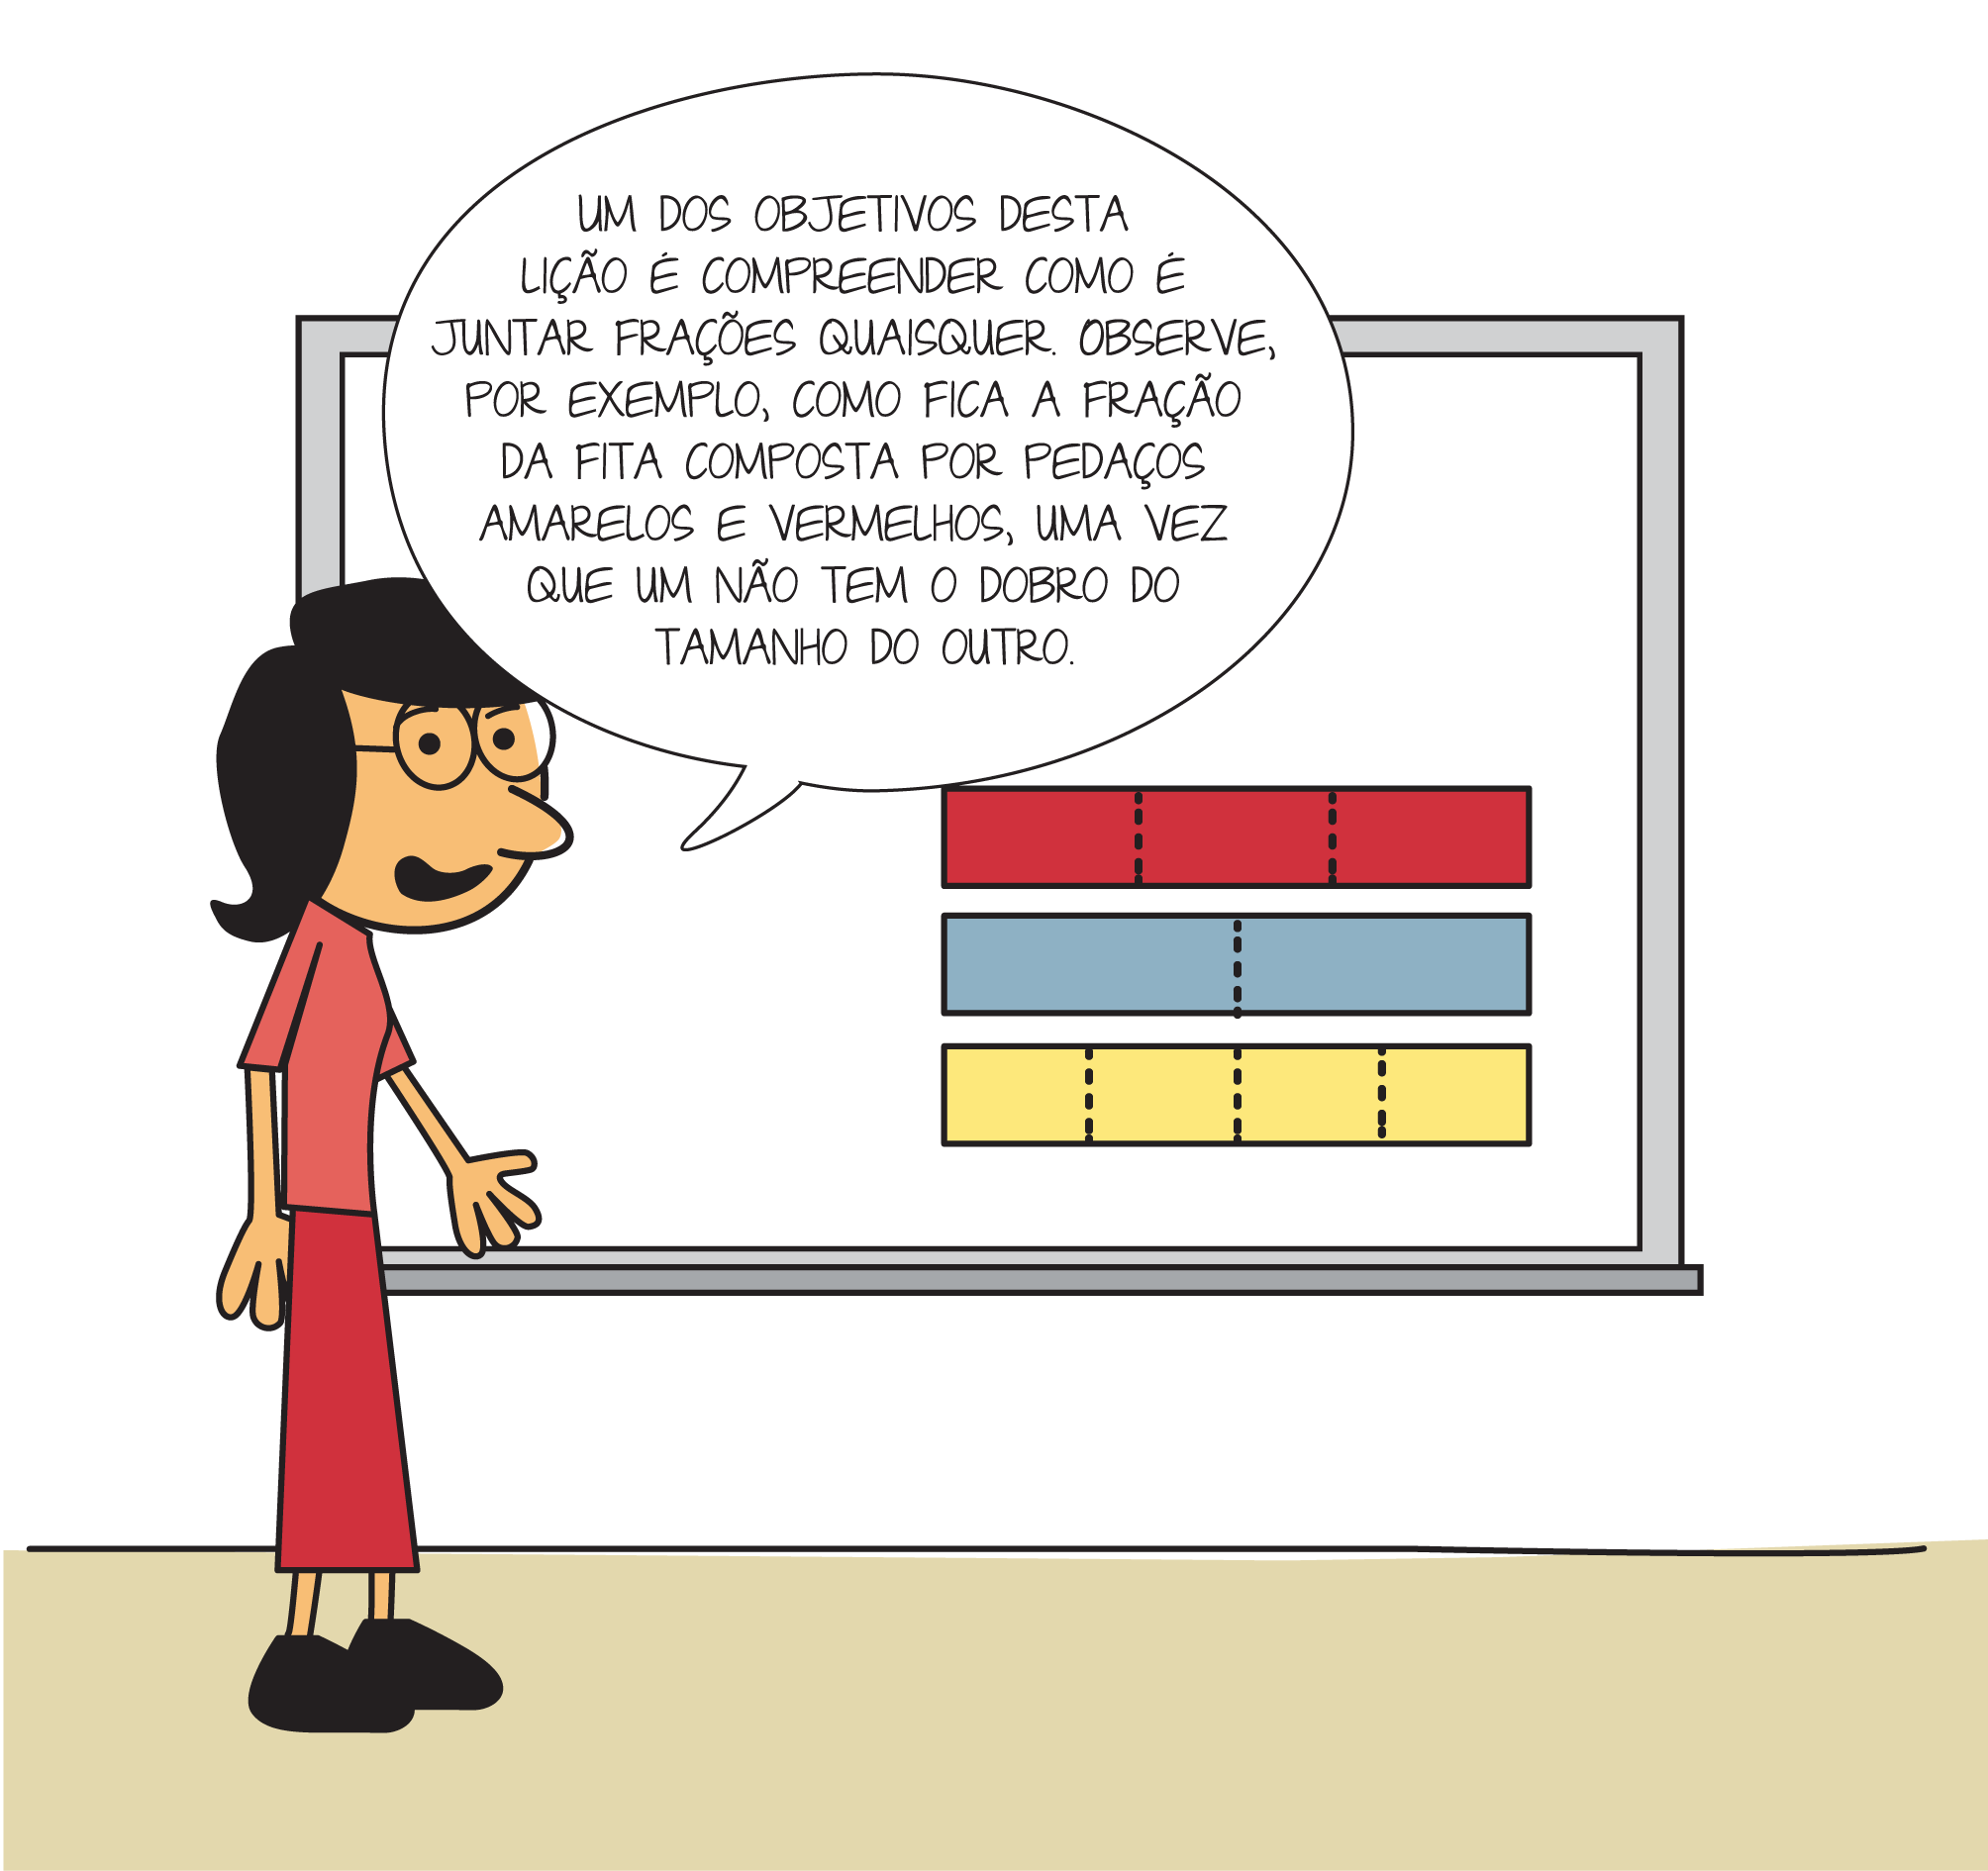
\includegraphics[width=330pt, keepaspectratio]{../figuras/licao05/ativ2_fig01.png}
%\end{center}


\begin{center}
	\begin{tikzpicture}[x=1.0cm,y=1.0cm, scale=.5]
	\draw[fill=light] (0.,0) rectangle (3,2);
	\draw[fill=common] (3,0) rectangle (9.,2.);
	%\draw[fill=light] (9,0) rectangle (12,2);
	\end{tikzpicture}
\end{center}

\end{atividade}

\begin{atividade}[label=chap5-ativ3]{}


Uma barra de chocolate é vendida com as marcações mostradas na figura abaixo.

 \begin{center}
 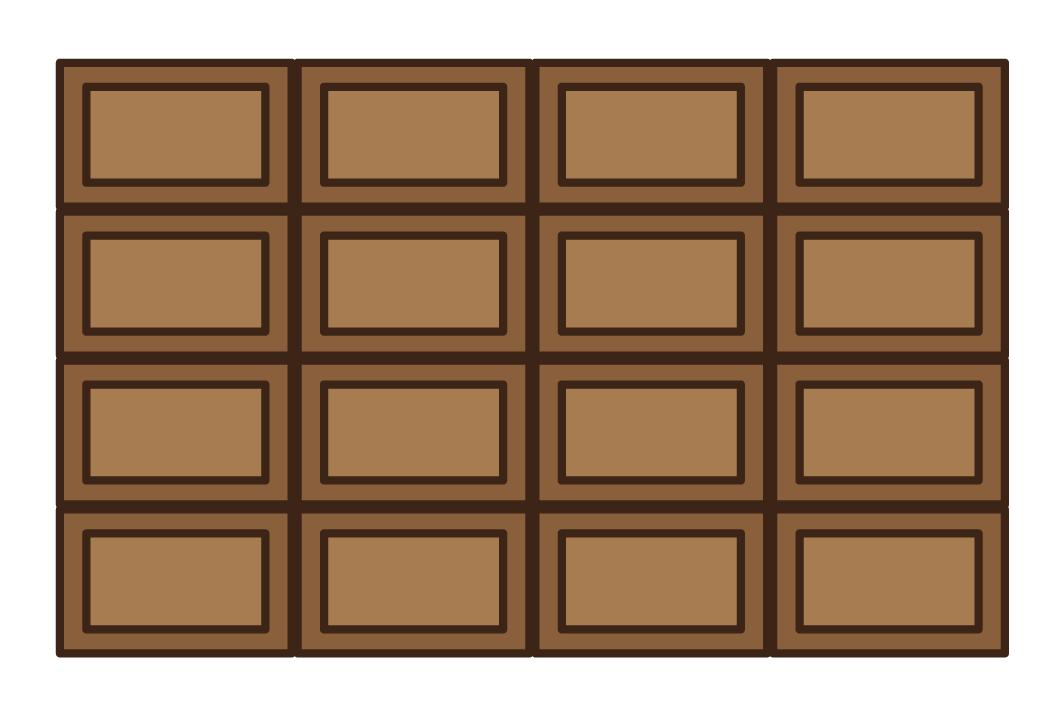
\includegraphics[width=150pt, keepaspectratio]{../figuras/licao05/ativ3_fig01.png}
 \end{center}


Alice comeu a metade dessa barra de chocolate (em bege) e Miguel quebrou o restante da barra em pedaços, seguindo as marcações e comeu 3 desses pedaços (em azul).

\begin{center}
\begin{tikzpicture}[x=1.0cm,y=1.0cm, scale=.7]
\fill[fill=light] (-1.,5.) -- (-1.,1.) -- (3.,1.) -- (3.,5.) -- cycle;
\fill[fill=common] (3.,5.) -- (5.,5.) -- (5.,3.) -- (3.,3.) -- cycle;
\fill[fill=common] (5.,5.) -- (7.,5.) -- (7.,4.) -- (5.,4.02) -- cycle;
\draw  (-1.,5.)-- (-1.,1.);
\draw  (-1.,1.)-- (3.,1.);
\draw  (3.,1.)-- (7.,1.);
\draw  (7.,1.)-- (7.,5.);
\draw  (7.,5.)-- (-1.,5.);
\draw  (3.,5.)-- (3.,3.);
\draw  (5.,5.)-- (5.,1.);
\draw  (-1.,3.)-- (7.,3.);
\draw  (-1.,2.)-- (7.,2.);
\draw  (1.,5.)-- (1.,1.);
\draw  (-1.,4.)-- (7.,4.);
\draw  (3.,3.)-- (3.,1.);
\end{tikzpicture}
\end{center}

Se considerarmos a barra de chocolate como a unidade, Alice comeu $\frac{1}{2}$ da barra e Miguel $\frac{3}{16}$. Cada pedaço da barra partida por Miguel corresponde a uma fração da barra. Observe que as quantidades de chocolate comidas por Alice e Miguel podem ser ambas escritas como junção dessas frações: Miguel comeu 3 desses pedaços e Alice 8.
\begin{enumerate}[a)]
\item Cada um dos pedaços partidos por Miguel corresponde a que fração da barra de chocolate?
\item Complete a parte em branco (numerador) para indicar a fração da barra de chocolate que Alice comeu.
$$\frac{1}{2} = \frac{\text{\Large $\square$} }{16}$$
\item Que fração da barra de chocolate foi comida por Alice e por Miguel, juntos?
\item  Que fração da barra de chocolate restou?
\end{enumerate}
\end{atividade}

\begin{atividade}[label=chap5-ativ4]{}


Amanda, Bruno e Caio pediram três pizzas do mesmo tamanho, mas com sabores diferentes. Todas as pizzas nessa pizzaria são servidas em {\bf 12 fatias} iguais. Amanda comeu $\frac{1}{6}$ de uma pizza, Bruno comeu $\frac{3}{4}$ de outra, e Caio comeu $\frac{2}{3}$ da pizza que pediu.

\begin{center}
\begin{tabular}{m{.3\textwidth}m{.3\textwidth}m{.3\textwidth}}

\begin{tikzpicture}
\fill[light, opacity = .8] (0,0) -- (30:20) arc (30:90:20) --cycle;
\foreach \x in {0,60,120}{ \draw (\x:20) -- (\x:-20);}
\foreach \x in {30,90,150}{ \draw[very thick, light] (\x:20) -- (\x:-20);}
\draw[|-|] (30:25) arc (30:90:25);
\node[] at (60:30) {$\dfrac{1}{6}$};
\draw (0,0) circle (20);
\end{tikzpicture}

&
\begin{tikzpicture}
\fill[common, opacity = .8] (0,0) -- (-180:20) arc (-180:90:20) --cycle;
\foreach \x in {0,30,60,120,150}{ \draw (\x:20) -- (\x:-20);}
\foreach \x in {0,90}{ \draw[very thick, common] (\x:20) -- (\x:-20);}
\draw[|-|] (0:25) arc (0:90:25);
\node[] at (45:30) {$\dfrac{1}{4}$};
\draw (0,0) circle (20);
\end{tikzpicture}
&
\begin{tikzpicture}
\fill[special, opacity = .8] (0,0) -- (-150:20) arc (-150:90:20) --cycle;
\foreach \x in {0,30,60,90,120,150}{ \draw (\x:20) -- (\x:-20);}
\foreach \x in {-30,90,210}{ \draw[very thick, special] (0,0) -- (\x:20);}
\draw[|-|] (-30:25) arc (-30:90:25);
\node[] at (30:30) {$\dfrac{1}{3}$};
\draw (0,0) circle (20);
\end{tikzpicture}
\\
 Fração de pizza consumida por Amanda $\frac{1}{6}$  & Fração de pizza consumida por Bruno $\frac{3}{4}$  & Fração de pizza consumida por Caio $\frac{2}{3}$
\end{tabular}
\end{center}

\begin{enumerate}[a)]
\item  Que fração de uma pizza cada fatia representa?
 \item Complete os espaços (numeradores) a seguir registrando outra representação para a fração de uma pizza que cada uma das crianças comeu.\\ Amanda: $\frac{1}{6} =\frac{}{12}  \quad \quad$ Bruno: $\frac{3}{4} =\frac{}{12} \quad \quad$ Caio: $\frac{2}{3} =\frac{}{12}$
 \item Quem comeu mais pizza? Quem comeu menos pizza?
 \item Que quantidade de pizza Bruno comeu a mais do que Caio?
 \item Que quantidade de pizza Amanda e Bruno comeram juntos?
  \item Que fração de uma pizza Amanda comeu a menos do que Caio?
  \item Quanto a mais de pizza Bruno consumiu, em relação a Amanda?
\end{enumerate}
\end{atividade}

\section{ORGANIZANDO AS IDEIAS }

Na \hyperref[chap5-ativ2]{Atividade 2}, juntou-se um pedaço de fita amarela com um pedaço azul. Para saber  que fração essa nova fita representa do tamanho original das fitas, deve-se somar $\frac{1}{2}$ e $\frac{1}{4}$, porque a fita azul é metade e a amarela é um quarto do tamanho original das fitas.

FIGURAS

Como somar metades e quartos? Para resolver esse problema,  subdivide-se o pedaço de fita azul em duas partes iguais, como na figura a seguir, obtendo-se assim dois quartos.

FIGURAS

Somar $\frac{2}{4}$ com $\frac{1}{4}$ é mais simples: $\frac{2}{4} + \frac{1}{4} = \frac{3}{4}$.

Repare que essa também foi a estratégia usada para somar as quantidades de chocolate comidas por Alice ($\frac{1}{2}$ de uma barra) e por Miguel ($\frac{3}{16}$ de uma barra), uma vez que $\frac{1}{2}$ e $\frac{3}{16}$ têm denominadores diferentes. 
Observou-se que metade da barra de chocolate corresponde a $\frac{8}{16}$ dessa barra. 
Somar $\frac{8}{16}$ com $\frac{3}{16}$ é simples: $\frac{8}{16} + \frac{3}{16} = \frac{11}{16}$. 

FIGURA

Para se calcular quanto chocolate restou foi necessário retirar $\frac{11}{16}$ da unidade, isto é, $1 - \frac{11}{16}$. 
Novamente deve-se representar as quantidades por frações com o mesmo denominador. 
Para isso observa-se que a barra de chocolate está subdividida em 16 partes iguais, ou seja,  $1 = \frac{16}{16}$. Assim, escreve-se $\frac{16}{16} - \frac{11}{16} = \frac{5}{16}$. 
Restando, portanto, $\frac{5}{16}$ da barra de chocolate.

Na \hyperref[chap5-ativ4]{Atividade 4}, para calcular a fração de uma pizza que Bruno e Caio comeram juntos, foi necessário calcular $\frac{3}{4} + \frac{2}{3}$. 
Agora surge outra novidade, além dos denominadores serem diferentes, não é possível igualar os denominadores alterando apenas uma das frações.

FIGURA

Subdividindo-se  a pizza em 12 fatias iguais, as quantidades $\frac{3}{4}$ e $\frac{2}{3}$ podem ser representadas com frações de mesmo denominador: $\frac{3}{4} = \frac{9}{12}$ e $\frac{2}{3} = \frac{8}{12}$. Assim,

\[ \frac{3}{4} + \frac{2}{3} = \frac{9}{12} + \frac{8}{12} = \frac{17}{12}\]

de uma pizza ou $1$ pizza inteira e $5$ doze avos de uma pizza pois 

\[\frac{17}{12} = \frac{12}{12} + \frac{5}{12} = 1 + \frac{5}{12}.\]

A escolha adequada de uma subdivisão da unidade que permita representar as frações com um mesmo denominador foi a estratégia usada para calcular a adição e a subtração de frações. 
Essa será a estratégia geral para se efetuar adição e subtração de frações.

Repare que pode haver mais do que uma subdivisão comum da unidade, por exemplo

\[ \frac{1}{6} + \frac{3}{4}  = \frac{2}{12} + \frac{9}{12}  = \frac{11}{12}.\]

FIGURAS

Mas também $\frac{1}{6} + \frac{3}{4} = \frac{4}{24} + \frac{18}{24} = \frac{22}{24}$.

FIGURAS

ou ainda, $\frac{1}{6} + \frac{3}{4} = \frac{6}{36} + \frac{27}{36} = \frac{33}{36}$

FIGURA

e, como se sabe, $\frac{11}{12} = \frac{22}{24} = \frac{33}{36}$.


\section{MÃO NA MASSA }

\begin{atividade}{}

Os dois retângulos da figura a seguir são iguais. 
Em um deles está representada a fração $\frac{3}{5}$ e no outro a fração $\frac{7}{10}$ do retângulo.

\begin{center}
\begin{tikzpicture}[scale=4]
\fill[fill=common, fill opacity=.3] (0,0) rectangle (10,5);
\fill[attention] (0,0) rectangle (6,5);
\draw (0,0) rectangle (10,5);
\foreach \x in {2,4,...,8} \draw (\x,0) -- (\x, 5);

\begin{scope}[shift={(14,0)}]
\fill[fill=common, fill opacity=.3] (8,2.5) rectangle (10,5);
\fill[fill=common, fill opacity=.3] (6,0) rectangle (10,2.5);
\fill[light] (0,0) rectangle (6,5);
\fill[light] (6,2.5) rectangle (8,5);
\draw (0,0) rectangle (10,5);
\foreach \x in {2,4,...,8} \draw (\x,0) -- (\x, 5);
\draw (0,2.5) -- (10, 2.5);
\end{scope}
\end{tikzpicture}
\end{center}

\begin{enumerate} [\quad a)] %s
  \item     Determine uma subdivisão da unidade que permita expressar essas quantidades por frações com um mesmo denominador. Represente tal subdivisão nas figuras acima.
  \item     Escreva frações iguais a     $\frac{3}{5}$     e a     $\frac{7}{10}$     a partir dessa subdivisão.
  \item     Existe alguma outra subdivisão, diferente da que você usou para responder os itens a) e b), com a qual também seja possível responder ao item b)? Se sim, qual?
  \item     Juntas, as regiões destacadas em vermelho e em laranja determinam um região maior, menor ou igual a um retângulo? Explique.
\end{enumerate} %s
\end{atividade}

\begin{atividade}{}

Aqui retomamos a \hyperref[chap5-ativ2]{Atividade 2}, na qual a professora Estela comprou fitas de mesmo tamanho e as cortou em partes iguais: a vermelha em três pedaços; a azul em dois pedaços e a amarela em quatro pedaços.

\begin{center}
\begin{tikzpicture}[x=1.0cm,y=1.0cm, scale=.5]
\draw[fill=attention] (0.,1) rectangle (12.,3.);
\foreach \x in {4,8} \draw[dashed] (\x,1) -- (\x,3);
\draw[fill=common] (0.,-2) rectangle (12.,0.);
\draw[dashed] (6,-2) -- (6,0);
\draw[fill=light] (0.,-5) rectangle (12.,-3.);
\foreach \x in {3,6,9} \draw[dashed] (\x,-5) -- (\x,-3);
\end{tikzpicture}
\end{center}

\begin{enumerate}[a)]
  \item  Agora, a professora Estela juntou um pedaço da fita vermelha com um pedaço da fita azul. Essa nova fita formada tem tamanho maior, menor ou igual ao tamanho original de uma fita? A que fração de uma fita original corresponde a nova fita vermelha e azul? Qual é a diferença entre os tamanhos de uma fita original e da fita vermelha e azul?
  \item  A professora formou então mais uma fita colorida, agora juntando, de forma intercalada, dois pedaços vermelhos e três pedaços amarelos. Essa nova fita vermelha e amarela é maior ou menor do que uma fita original? A que fração de uma fita original corresponde a nova fita vermelha e amarela? Qual é a diferença entre os tamanhos da fita original e da fita vermelha e amarela?
\end{enumerate}

\end{atividade}

\begin{atividade}{}


Nos itens a seguir, escreva frações que tenham mesmo denominador e são iguais a cada uma das frações dadas.
Para cada par de frações, destaque a subdivisão escolhida da unidade para determinar o denominador comum e represente essa subdivisão por meio de um desenho.

\begin{center}
  \begin{tabular}{m{0.25\textwidth}m{0.25\textwidth}m{0.25\textwidth}}

     a) $\frac{1}{3}$ e $\frac{2}{9}$  &   b) $\frac{3}{10}$ e $\frac{4}{5}$  &   c) 1 e $\frac{3}{7}$  \\
     \\
     d) $\frac{3}{5}$ e $\frac{8}{3}$  &   e) $\frac{7}{8}$ e $\frac{13}{12}$  &  f) $\frac{7}{4}$ e 5
  \end{tabular}
\end{center}
\end{atividade}

\begin{atividade}{}

Em cada um dos itens a seguir, determine o resultado e explique seu raciocínio por meio de desenhos.

\begin{center}
  \begin{tabular}{m{0.25\textwidth}m{0.25\textwidth}m{0.25\textwidth}}
     a) $\frac{1}{3} - \frac{2}{9}$  &   b) $\frac{3}{10} + \frac{4}{5}$  &   c) $1 - \frac{3}{7}$
  \end{tabular}
\end{center}
\end{atividade}

\begin{atividade}{}
	Para determinar a soma $2 + \frac{1}{3}$ Miguel inicialmente marcou na reta numérica o ponto determinado pela justaposição do segmento correspondente a $2$ unidades com um segmento igual a $\frac{1}{3}$ da unidade, como na figura a seguir.

Miguel relacionou essa estratégia com o seguinte cálculo:
\[ 2 + \frac{1}{3} =  \frac{6}{3} + \frac{1}{3} = \frac{7}{3}\]

%
% \begin{center}
%  \begin{tikzpicture}[x=17mm,y=17mm]
%   \draw[->] (0,-.25) -- (0,3.25);
%   \foreach \x in {0,...,3}{
%   \draw (-3pt,\x)--(3pt,\x);
%   \node at (-7pt,\x) {\x};}
%  \foreach \x in {2+1/3,2+2/3}\draw (-2pt,\x)--(2pt,\x);
%  \draw[|-|] (9pt,2) -- (9pt,2+1/3);
%  \node at (20pt,2+1/6) {$\dfrac{1}{3}$};
%  \draw[->] (-35pt,2+1/3) -- (-9pt,2+1/3);
%  \node at (-1.1,2+1/3) {$2 + \dfrac{1}{3}$};
%  \fill[common] (0,2+1/3) circle (3pt);
%  \end{tikzpicture}
% \end{center}


\begin{center}
 \begin{tikzpicture}[x=17mm,y=17mm]
  \draw[->] (0,-.25) -- (0,3.25);
  \foreach \x in {0,...,3}{
  \draw (-3pt,\x)--(3pt,\x);
  \node at (-7pt,\x) {\x};}
 \foreach \x in {2+1/3,2+2/3}\draw (-2pt,\x)--(2pt,\x);
 \draw[|-|] (9pt,2) -- (9pt,2+1/3);
 \node at (20pt,2+1/6) {$\dfrac{1}{3}$};
 \draw[->] (-35pt,2+1/3) -- (-9pt,2+1/3);
 \node at (-1.1,2+1/3) {$2 + \dfrac{1}{3}$};
 \fill[common] (0,2+1/3) circle (3pt);
 \draw[dotted] (9 pt, 2+1/3) -- (1.9, 2+1/3);

 \begin{scope}[shift={(2,0)}]
 %reta numerica vertical
 \draw[->] (0,-.25) -- (0,3.25);
  \foreach \x in {0,...,3}{
  \draw (-3pt,\x)--(3pt,\x);
  \node at (-7pt,\x) {\x};}
\foreach \x in {0,.3333,...,2.6666}\draw (-2pt,\x)--(2pt,\x);
  \fill[common] (0,2+1/3) circle (3pt);

% segmentos de 1/3 ao lado da reta

\foreach \x in {1,...,6}{
\draw[|-|] (9pt,\x/3+.01) -- (9pt,\x/3+1/3-.01);
\node at (20pt,\x/3+1/6) {{\small $\frac{1}{3}$}};}
\draw[|-|] (9pt,0) -- (9pt,1/3-.01);
\node at (20pt,1/6) {{\small $\frac{1}{3}$}};

%flecha e texto.
\draw[<-]  (30 pt, 2+1/6) -- (56pt, 2+1/6);
\node at (90pt, 2+1/6) {1 fração de $\dfrac{1}{3}$};
\node at (90pt, 1.6) {$+$};
\node at (90pt, 1) {6 frações de $\dfrac{1}{3}$};
%linhas tracejadas e chave
\foreach \x in {0,2} \draw[dotted] (25pt,\x) -- (45pt,\x);
\draw [thick, decoration={brace,mirror,raise=5}, decorate] (45pt,0) -- (45pt,2);
 \end{scope}
 \end{tikzpicture}
\end{center}

\begin{enumerate}[a)]
 \item Em cada item a seguir, a partir da imagem repita o procedimento feito por Miguel e realize os cálculos.

\begin{center}
\begin{tabular}{m{.3\textwidth}m{.3\textwidth}m{.3\textwidth}}
 (A) & (B) & (C)\\

 \begin{tikzpicture}[x=17mm,y=17mm]
  \draw[->] (0,-.5) -- (0,4.5);
  \foreach \x in {0,...,4}{
  \draw (-3pt,\x)--(3pt,\x);
  \node at (-7pt,\x) {\x};}
 \foreach \x in {3.25,3.5,3.75}\draw (-2pt,\x)--(2pt,\x);
 \fill[common] (0,3.25) circle (3pt);

 % setinha e texto
 \draw[->] (-35pt,3.25) -- (-9pt,3.25);
 \node at (-1.1,3.25) {$3 + \dfrac{1}{4}$};

 \end{tikzpicture}
&

 \begin{tikzpicture}[x=17mm,y=17mm]
  \draw[->] (0,-.5) -- (0,5.5);
  \foreach \x in {0,...,5}{
  \draw (-3pt,\x)--(3pt,\x);
  \node at (-7pt,\x) {\x};}
 \draw (-2pt,4.5)--(2pt,4.5);
 \fill[common] (0,4.5) circle (3pt);

 % setinha e texto
 \draw[->] (-35pt,4.5) -- (-9pt,4.5);
 \node at (-1.1,4.5) {$4 + \dfrac{1}{2}$};
  \end{tikzpicture}
 &
 \begin{tikzpicture}[x=17mm,y=17mm]
  \draw[->] (0,-.5) -- (0,3.5);
  \foreach \x in {0,...,3}{
  \draw (-3pt,\x)--(3pt,\x);
  \node at (-7pt,\x) {\x};}
 \draw (-2pt,2.6)--(2pt,2.6);
 \foreach \x in {2.2,2.4,...,2.8}\draw (-2pt,\x)--(2pt,\x);
 \fill[common] (0,2.6) circle (3pt);

 % setinha e texto
 \draw[->] (-35pt,2.6) -- (-9pt,2.6);
 \node at (-1.1,2.6) {$2 + \dfrac{3}{5}$};

 \end{tikzpicture}
\end{tabular}
\end{center}

 \item Que valor é obtido se juntarmos 7 inteiros com dois terços?
\end{enumerate}
\end{atividade}

\begin{atividade}{}


Quanto se deve acrescentar a $\frac{3}{8}$ para que se obtenha $\frac{27}{8}$?

\end{atividade}

\begin{atividade}{}

Qual é o maior número, $\frac{19}{7}$ ou $2$? Quanto deve acrescentado ao menor número para se chegar ao maior?

\end{atividade}

\begin{atividade}{}

Observando a reta, Miguel conseguiu determinar o tamanho do segmento azul entre os dois pontos $A = 3$ e $B = 7$ marcados da seguinte forma:

\begin{center}
\definecolor{DarkGreen}{rgb}{0.0, 0.5, 0.0}
\begin{tikzpicture}[x=17mm,y=17mm]
\draw[->] (-0.5,0) -- (7.5,0) ; %reta anterior
\foreach \x in {0,...,7}{ \draw (\x,3pt) -- (\x,-3pt) node[below] {\x}; }
\draw[common, line width=0.4mm] (3,0) -- (7,0);
\foreach \x in {3,7} \fill[common] (\x,0) circle (3 pt);
\node[above] at (3,3pt) {$A$};
\node[above] at (7,3pt) {$B$};
\node[color=attention] at (5,-30pt) {{\Large 7}};
\node[] at (5.2,-30pt) {{\Large $-$}};
\node[color=DarkGreen] at (5.4,-30pt) {{\Large 3}};
\node[] at (5.6,-30pt) {{\Large $=$}};
\node[common] at (5.8,-30pt) {{\Large 4}};
\draw[|-|, shift={(0,-30pt)},  color=DarkGreen, line width=0.4mm] (0,0)--(3,0);
\draw[|-|, shift={(0,-45pt)}, color=attention, line width=0.4mm] (0,0)--(7,0);
\end{tikzpicture}
\end{center}

Miguel calculou o tamanho do segmento azul fazendo a diferença entre o tamanho do segmento vermelho e o tamanho do segmento verde. Assim, concluiu que o tamanho do segmento AB é igual a 4.
Usando um raciocínio parecido, e considerando $C = \frac{5}{4}$ e $D=\frac{11}{6}$, ajude Miguel a realizar as tarefas a seguir.

\begin{center}
\begin{tikzpicture}[x=50mm,y=50mm]
\draw[->] (-0.25,0) -- (2.25,0) ; %reta anterior
\foreach \x in {0,1,2}{ \draw (\x,3pt) -- (\x,-3pt) node[below] {\x}; }
\draw[common, line width=0.4mm] (5/4,0) -- (11/6,0);
\foreach \x in {5/4,11/6} \fill[common] (\x,0) circle (3 pt);
\node[above] at (5/4,3pt) {$C$};
\node[above] at (11/6,3pt) {$D$};
\node[below] at (5/4,-3pt) {$\frac{5}{4}$};
\node[below] at (11/6,-3pt) {$\frac{11}{6}$};
\end{tikzpicture}
\end{center}

\begin{enumerate} [\quad a)] %s
  \item     Escreva $C$ e $D$ a partir de uma mesma subdivisão da unidade (isto é, com o mesmo denominador).
  \item     Determine seis frações que correspondam a pontos na reta numérica entre $C$ e $D$. \newline
  Discuta com seus colegas se é possível determinar mais que seis frações e, se for possível, quais seriam as estratégias para fazer isso.
  \item     Calcule o tamanho do segmento     $CD$.
  \item     Determine uma fração que, somada a     $\frac{5}{4}$     dê um resultado menor que     $\frac{11}{6}$. Justifique a sua resposta usando a reta.     $$ \dfrac{5}{4} +\dfrac{\text{\Large $\square$}}{\text{\Large $\square$}} < \dfrac{11}{6}.$$
  \item     Determine outras três possíveis respostas para o item anterior.
  \item     Determine duas frações tais que a soma delas adicionada a $\frac{5}{4}$ dê como resultado $\frac{11}{6}$.
   Justifique a sua resposta usando a reta.     
   \[ \dfrac{5}{4} +\dfrac{\text{\Large $\square$}}{\text{\Large $\square$}} + \dfrac{\text{\Large $\square$}}{\text{\Large $\square$}} = \dfrac{11}{6}.\]
\end{enumerate} %s
\end{atividade}

\begin{atividade}{}

A família de Miguel reservou um determinado espaço retangular para fazer um canteiro em seu quintal. A família quer que o canteiro tenha rosas e verduras frescas. O pai de Miguel disse que precisa de $\frac{2}{3}$ do espaço inicialmente reservado, para cultivar rosas. A mãe disse que necessita de $\frac{1}{2}$ desse espaço, para plantar as verduras. Quando Miguel ouviu o diálogo dos pais, pensou nas seguintes questões:
\begin{enumerate} [\quad a)] %s
  \item     Quem precisa de mais espaço, seu pai ou sua mãe?
  \item     O espaço reservado inicialmente para o canteiro é suficiente para comportar os espaços de que o pai e a mãe de Miguel precisam?
  \item     Caso o espaço seja suficiente, que fração do canteiro ficaria sem uso?
  \item     Caso o espaço não seja suficiente, que fração do canteiro reservado inicialmente deverá ser acrescentada ao mesmo para que a família consiga fazer as plantações que deseja?
\end{enumerate} %s


Faça um desenho que ajude a explicar as suas respostas para as questões de Miguel. Não deixe de indicar a subdivisão da unidade que você empregou.
\end{atividade}

\begin{atividade}{}

Há três jarras de mesmo tamanho contendo água. 
Na primeira jarra, a água ocupa dois terços de sua capacidade. 
Na segunda, a água ocupa metade de sua capacidade. 
Na terceira, cinco oitavos.

%retirar os tracinhos da figura.
\begin{center}
  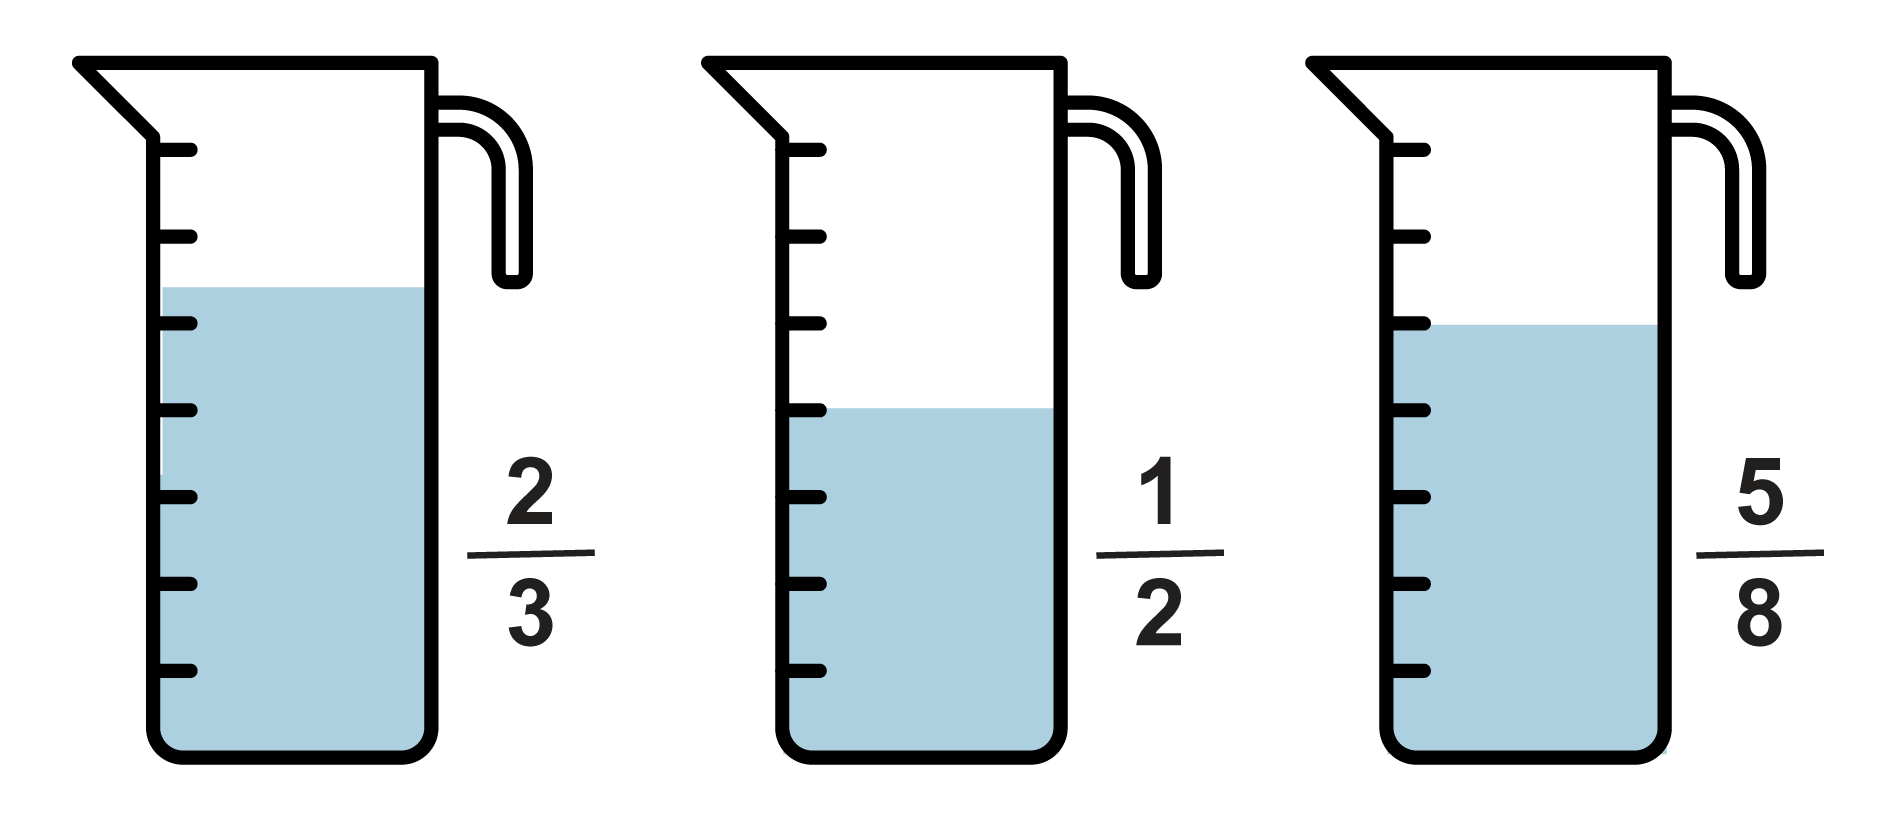
\includegraphics[width=280pt, keepaspectratio]{../figuras/licao05/ativ14_fig01.png}
\end{center}

É possível redistribuir a água de todos os recipientes em somente dois deles?
\end{atividade}

\section{QUEBRANDO A CUCA }


\begin{atividade}{}

Diga se as afirmações a seguir são verdadeiras ou falsas. Para as verdadeiras, explique com as suas palavras por que acha que são verdadeiras. Para as falsas, dê um exemplo que justifique a sua avaliação.
\begin{enumerate} [\quad a)] %s
  \item     Adicionando um número natural com uma fração que não é igual a um número natural obtemos como resposta um número natural.
  \item     Subtraindo de  um número natural  uma fração que não é igual a um número natural obtemos como resposta um número natural. 
  \item     Adicionando duas frações que não são iguais a um número natural nunca obtemos como resposta um número natural.
  \item     Subtraindo de uma fração que não é igual a um número natural outra fração que não é igual a um número natural nunca obtemos como resposta um número natural. 
\end{enumerate} %s
\end{atividade}

%%% Local Variables: 
%%% mode: latex
%%% TeX-master: "livro_aluno_completo.tex"
%%% End: 